\setauthor{Abdulrahman Al Sabagh}
\section{Strapi}
Strapi ist ein Headless \textbf{C}ontent \textbf{M}anagment \textbf{S}ystem (CMS),
welches eine vorgefertigte Benutzeroberfläche für Content-Creator
und auch für die Entwickler bereitstellt.

Mit der Verwendung davon sind Inhalte und dazu gebrauchte technische Funktionalitäten
sehr einfach erstellbar.
\cite{strapi-vs-wordpress}


\subsection*{Welche eingebauten Funktionalitäten bietet Strapi für Entwickler und Content-Manager}


Für die Entwickler werden folgende Funktionalitäten:

\begin{itemize}
    \item Fertige REST-Schnittstellen
    \item Qraphql Schnittstellen
    \item Eine Benutzeroberfläche, wo die Struktur und das Datenmodell einer Datenbank definieren kann
    \item Eine eingebaute JWT Authentifizierung
    \item File Upload
    \item Query Engine API
    \item Entity Service API
    \item Internationalisierungsplugin
    \item Plugin Store, wo man sehr viele hilfreiche Plugins wie zum Beispiel OpenAPI installieren kann
    \item Authorisierung und Rollenmanagement
\end{itemize}

\subsection{REST-Schnittstellen}
Für jedes Model werden die benötigten GET, POST, PUT und DELETE REST-Schnittstellen per default erstellt.
Jede Enpoint unterstützt auch eine Menge von unterschiedlichen Parametern, welche den Aufbau von dem Responsebody steuern können wie zum Beispiel.: filters, populate  und fields.
\cite{rest-query-parameters}
\subsection{Definierung von Datenstruktur und Datenmodell}

Mit der Verwendung dieser Oberfläche kann man folgende Elemente erstellen:
\begin{itemize}
    \item Collection Types
    \item Single Types
    \item Components
\end{itemize}

\subsubsection{Collection Types}

'Collection types are content-types that can manage several entries.'
\cite{collection-types}

Man kann also sagen, dass man mit der Verwendung von diesen Collection Types die Struktur einer Tabelle bzw. einer Collection definieren kann.
Allerdings schaut die Struktur der definierten SQL-Tabelle oder NoSQL-Collection nicht eins zu eins zu der Collection Type aus.
Die speziellen Datentype wie Files oder Custom Components werden nicht in der Datenbank als eine Tabellenspalte gespeichert.
Stattdessen werden die spezielle Typen in einer anderen Tabelle gespeichert, welche die Daten bei einem GET-Request der Endpoint  auf des erstellten Model, die Daten zur Verfügung stellt.

Folgende Datentypen  werden von Strapi zur Verfügung gestellt:

\begin{figure}[H]
    \centering
    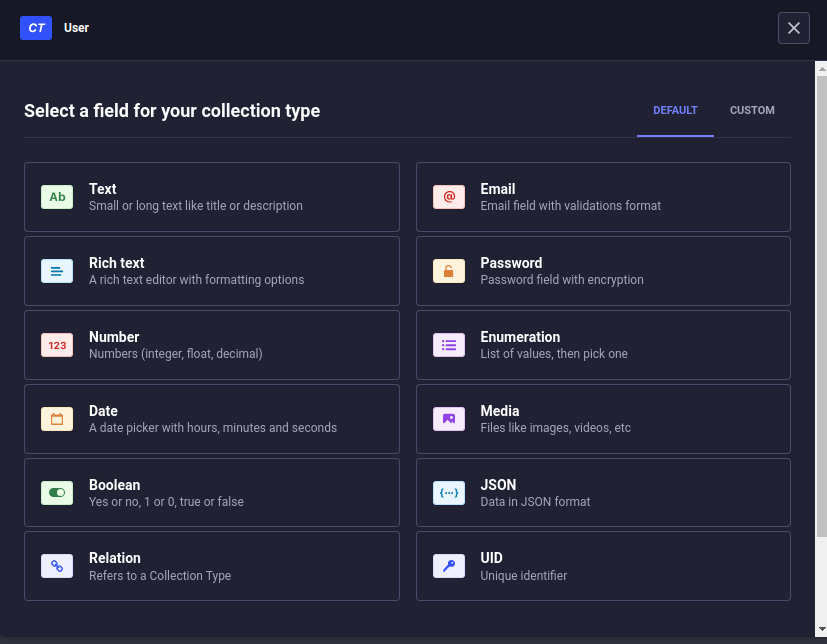
\includegraphics[width=\textwidth]{./pics/datatypes}
    \caption{Datentypen}
    \label{datatypes}
\end{figure}

Die Relationen zu anderen 'Collection Types' werden von Strapi als ein Datentyp interpretiert.
Dieser unterstützt die Standardbeziehungen einer Relationen Datenkbank zusätzlich zu bidirektionalen Beziehungen.
Bei den 'Many to Many' Beziehungen ist die Erstellung von einem zusätzlichen Collection Type, welcher als eine Assoziationstabelle dient, gar nicht nötig.
Die Assoziationstabellen werden von Strapi im Hintergrund erstellt.

\begin{figure}[H]
    \centering
    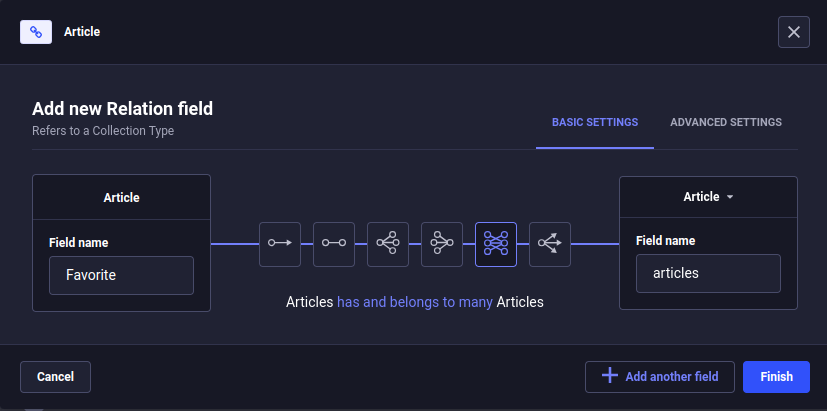
\includegraphics[width=\textwidth]{./pics/relations}
    \caption{Relationen}
    \label{relations}
\end{figure}


Zusätzlich zu der Erstellung von Spalten, haben Collection Types auch eine eingebaute Validierung, die man aktivieren kann.
\begin{figure}[H]
    \centering
    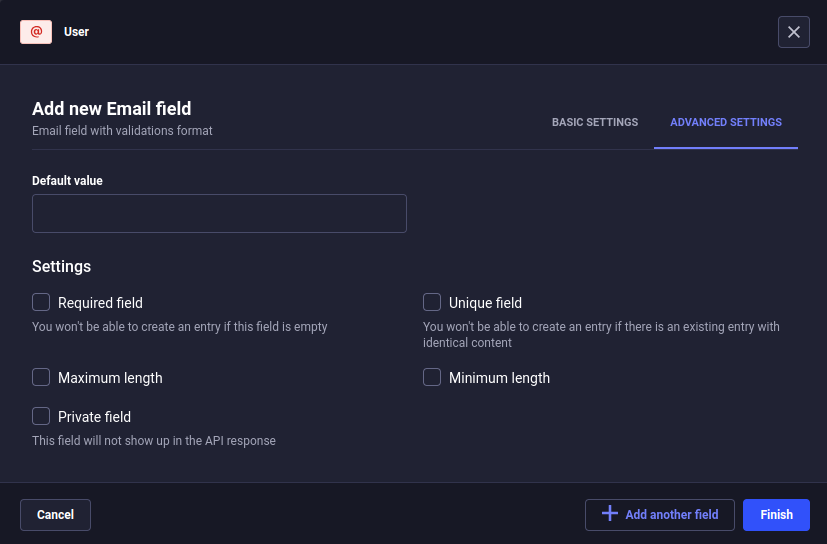
\includegraphics[width=\textwidth]{./pics/validation.png}
    \caption{validation}
    \label{validation}

\end{figure}

\subsubsection{Single Types}
'Single types are content-types that can only manage one entry'
\cite{collection-types}

\subsubsection*{Components}
'Components are a data structure that can be used in multiple collection types and single types.'
\cite{collection-types}

\subsection{Query Engine API}
'The Strapi backend provides a Query Engine API to interact with the database layer at a lower level.
The Query Engine API should mostly be used by plugin developers and developers adding custom business logic
to their applications.'
\cite{query-engine-api}

Diese ist mehr oder weniger wie ein \textbf{O}bject \textbf{R}elational \textbf{M}apper (ORM) oder ein Query Builder, wo man SQL oder NoSQL Queries aus einem JS Code generieren kann. Die selektierte Spalten werden dann in JS-Objekten serialisiert.

\subsection{Entity Service API}
'The Strapi backend provides an Entity Service API, built on top of the Query Engine API. The Entity Service is the layer that handles Strapi's complex data structures like components and dynamic zones, and uses the Query Engine API under the hood to execute database queries.'
Der Unterschiede zwischen dieses Service und die Query Engine API liegt dabei, dass die Entity Service API nicht nur die SQL bzw. NoSQL Struktur einer Tabelle bwz. einer Collection abfragt, sondern auch die anderen Typen, die in dem Collection Type gespeichert sind wie zum Beispiel File oder Custom Components, abfragen kann.
\cite{service-engine-api}
\subsection{File Upload}

Dabei ist das Wichtige, dass man Strapi so konfigurieren kann, dass er die Uploads für mehrere Bildschirme anpassen kann.
\begin{lstlisting}[caption=file upload config in strapi]
    export default ({ env }) => ({
        upload: {
          config: {
            breakpoints: {
              xlarge: 1920,
              large: 1000,
              medium: 750,
              small: 500,
              xsmall: 64
            },
          },
        },
      });
    
\end{lstlisting}
Es gibt auch andere Standardeinstellungen für File Uplaod wie zum Beispiel die Bestimmung von der Größe eines Uploads
\cite{upload}

Für den Content-Manager
\begin{itemize}
    \item Eine Oberfläche, wo die Inhalte eingepflegt werden können
    \item Eine Media Library
\end{itemize}

Es aber noch anzumerken, dass diese Oberfläche nur im Dev Mode funktionieren kann. In der produktiven Umgebung sind werden die Struktur der Datenbank zwar angezeigt. Diese ist aber nicht editierbar.


\subsection{Media Library}

Diese ist mehr oder weniger eine UI, wo der Content-Manager den Verzeichness, wo alle Files und Assets gespeichert sind, steuern kann.
Es gibt bei dieser die Möglichkeit neue Assets hochzuladen, Unterordnern zu erstellen und die Assets in diese zu speichern, Assets löschen und umbennen und diese auch Zuschneiden.
Man kann die Files in der Media Library auch beliebig sortieren und nach diesen auch suchen
\cite{media-library}

% Beispiele dafür sind:

% \begin{itemize}
%     \item \textbf{RE}presentational \textbf{S}tate \textbf{T}ransfer (REST)- bzw. \textbf{G}raph \textbf{Q}uery \textbf{L}anguage (Graphql)-Schnittstellen
%     \item Logik für die Authentifizierung
%     \item \textbf{C}reate, \textbf{R}ead, \textbf{U}pdate und \textbf{D}elete (CRUD)
%           Funktionalitäten jeder Business Entität
% \end{itemize}


\section{Firebase App Distribution}

``
Firebase App Distribution macht die Verteilung
Ihrer Apps an vertrauenswürdige Tester problemlos. Indem Sie Ihre Apps schnell
auf die Geräte der Tester übertragen, können Sie frühzeitig und häufig
Feedback einholen.
Und wenn Sie Crashlytics in Ihren Apps verwenden, erhalten Sie automatisch Stabilitätsmetriken für alle Ihre Builds, sodass Sie wissen, wann Sie zur Auslieferung bereit sind.
''\cite{fire-base-app-distribution}

Der Vorteil von Firebase App Distribution ist,
dass man die Applikation auf dem eigenen Mobilegerät ausprobieren kann,
ohne die App auf dem Play Store bzw. App Store hochladen zu müssen.